\chapter{PCB}
\label{cha:intro}
通过仿真证明可以完整实现红外发射和接收任务,在此设计两块PCB板以将其实现。

\section{红外发射PCB板}
\begin{figure}[H] % use float package if you want it here
    \centering
    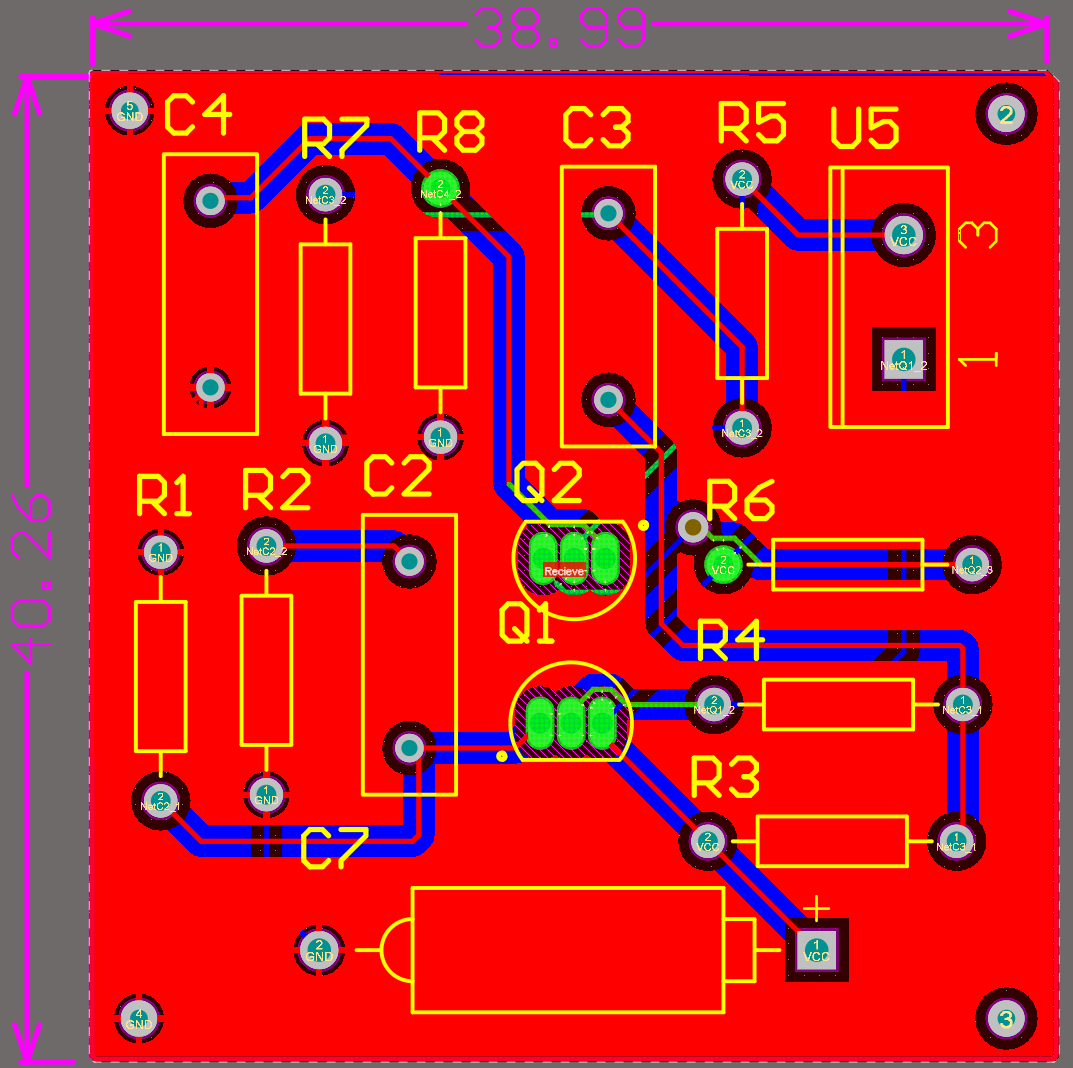
\includegraphics[width=1\textwidth]{6-1.png}
    \caption{Top Layer}
    \label{fig:xfig1}
\end{figure}

\begin{figure}[H] % use float package if you want it here
    \centering
    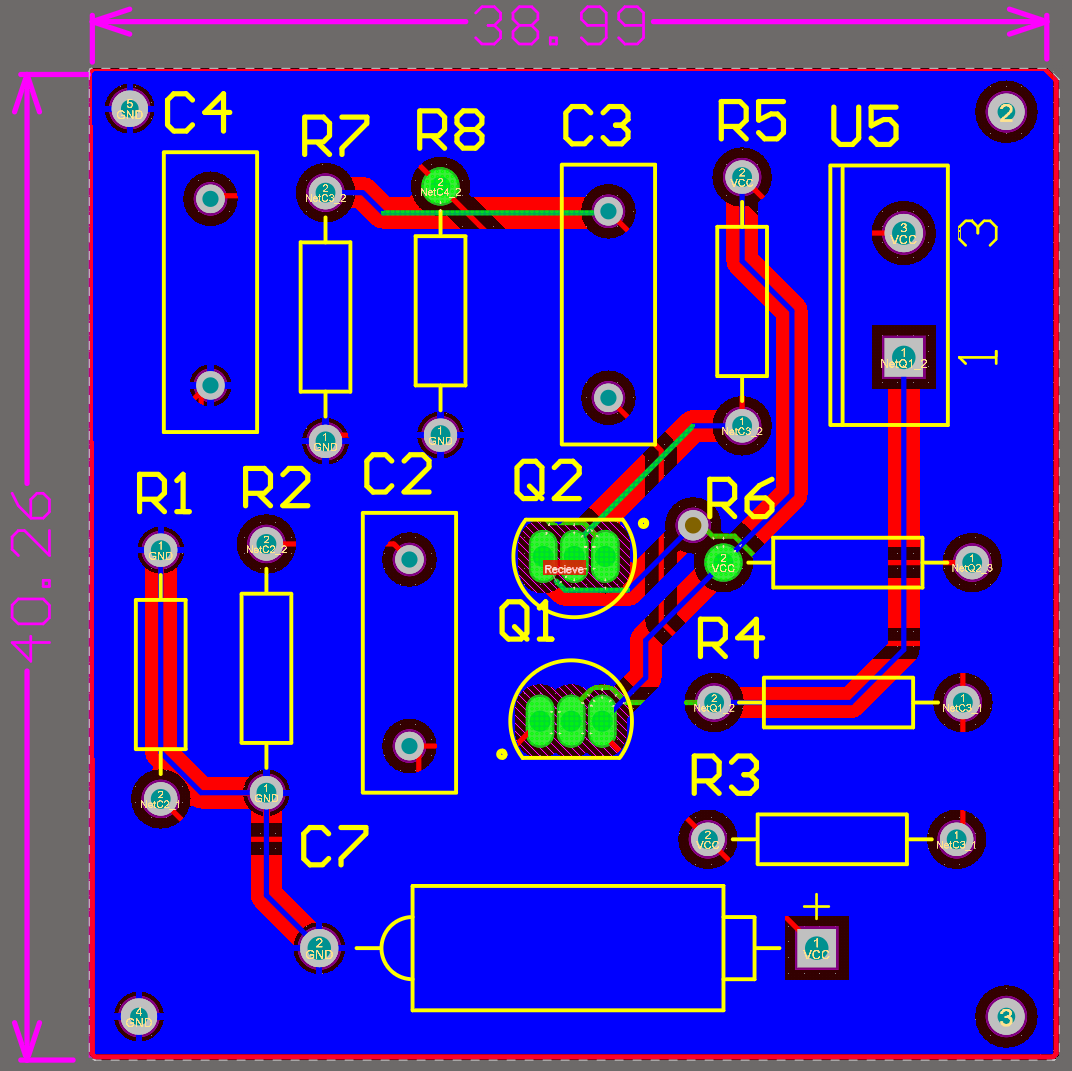
\includegraphics[width=1\textwidth]{6-3.png}
    \caption{Bottom Layer}
    \label{fig:xfig1}
 \end{figure}

 \section{红外接收PCB板}
 \begin{figure}[H] % use float package if you want it here
     \centering
     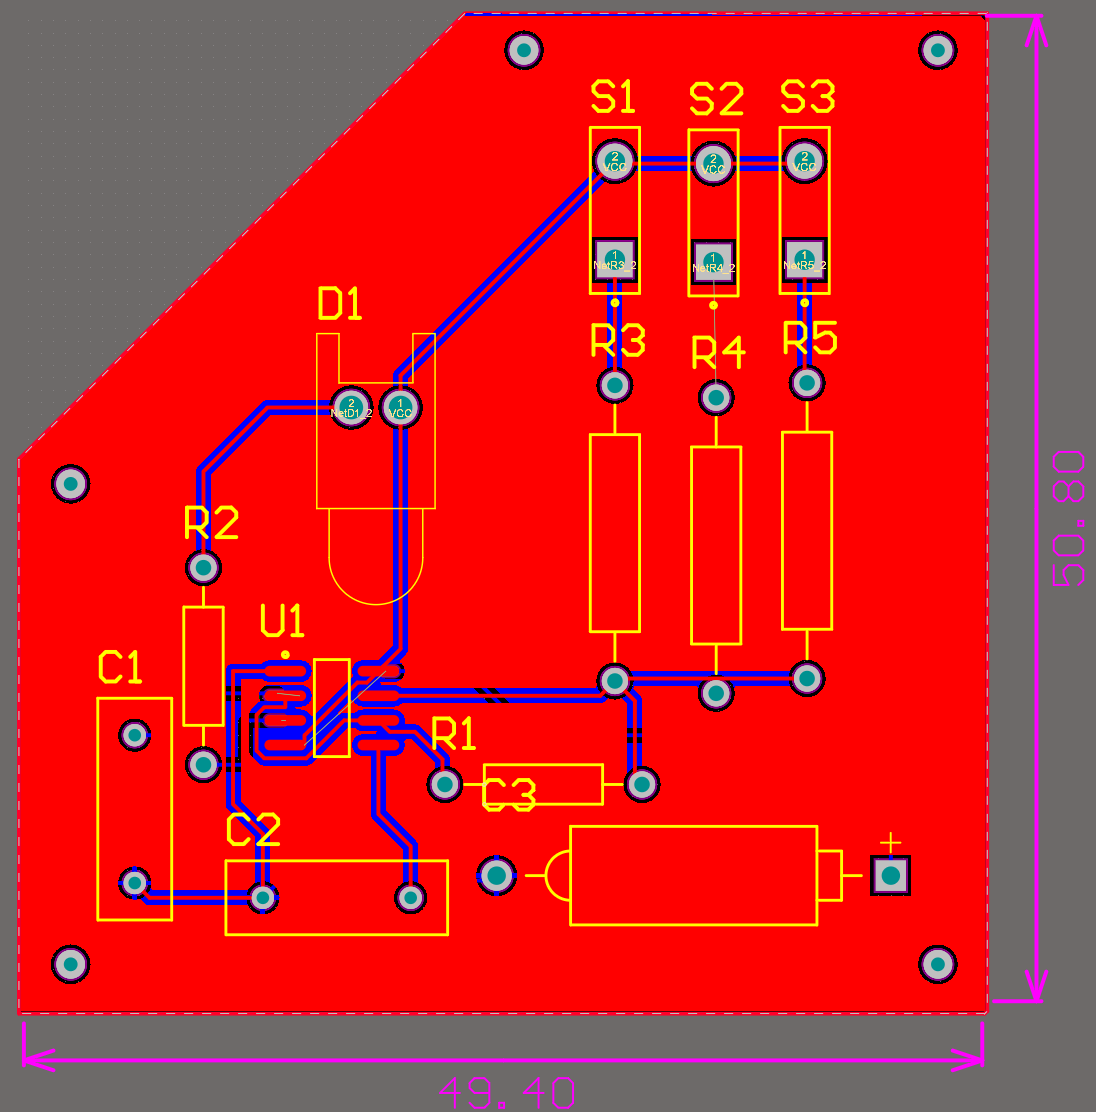
\includegraphics[width=1\textwidth]{6-2.png}
     \caption{Top Layer}
     \label{fig:xfig1}
 \end{figure}
 
 \begin{figure}[H] % use float package if you want it here
     \centering
     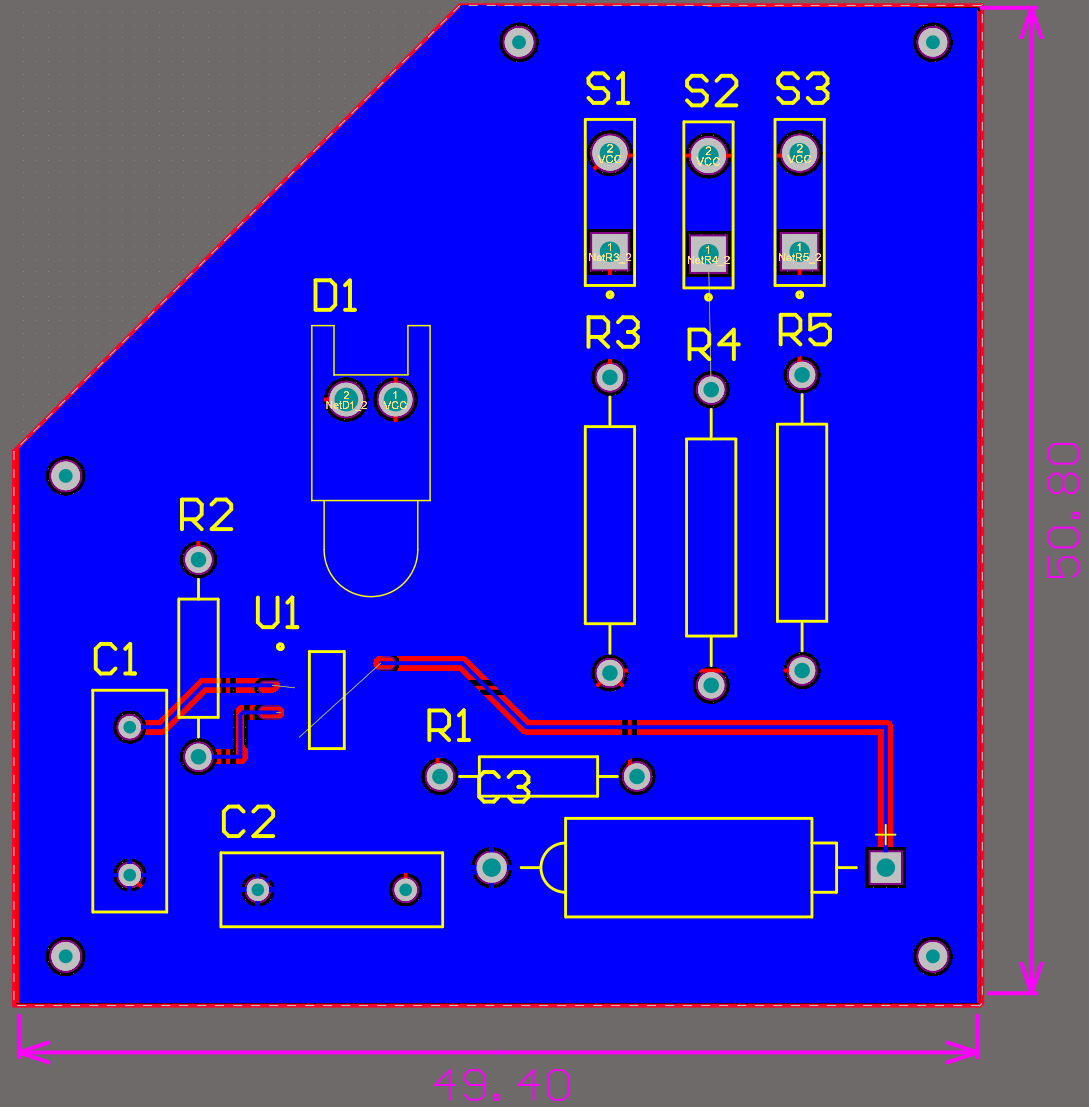
\includegraphics[width=1\textwidth]{6-4.png}
     \caption{Bottom Layer}
     \label{fig:xfig1}
  \end{figure}

\vspace{100pt}

\section{关键元器件参数}
NE555参数:
\begin{figure}[H] % use float package if you want it here
    \centering
    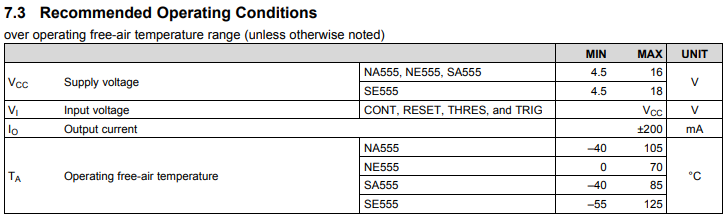
\includegraphics[width=1\textwidth]{NE555.png}
    \caption{NE555参数}
    \label{fig:xfig1}
 \end{figure}
 
2SC1815参数:
 \begin{figure}[H] % use float package if you want it here
     \centering
     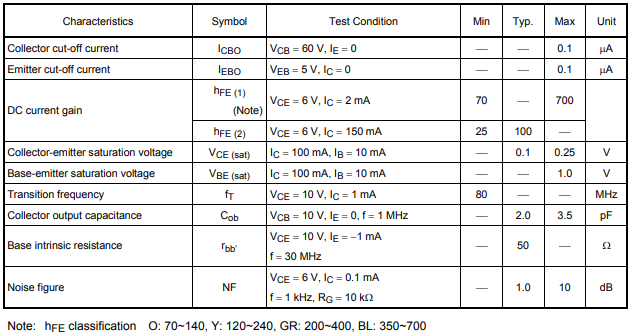
\includegraphics[width=1\textwidth]{2SC1815.png}
     \caption{2SC1815参数}
     \label{fig:xfig1}
  \end{figure}

BC848B参数:
\begin{figure}[H] % use float package if you want it here
    \centering
    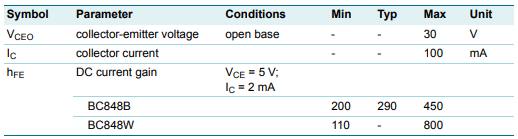
\includegraphics[width=1\textwidth]{BC848B.png}
    \caption{BC848B参数}
    \label{fig:xfig1}
 \end{figure}
\section{所有元器件列表}
\subsection{红外发射PCB板元器件列表}
\begin{figure}[H] % use float package if you want it here
    \centering
    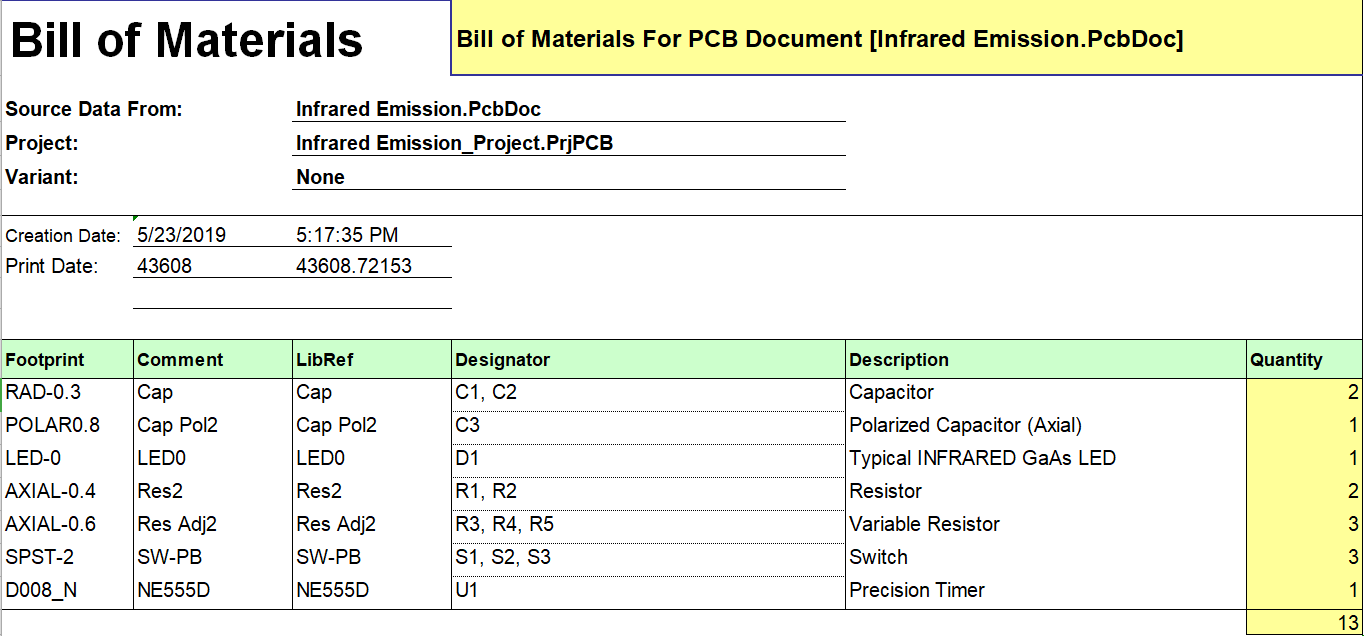
\includegraphics[width=1\textwidth]{7-1.png}
    \caption{红外发射PCB板元器件列表}
    \label{fig:xfig1}
 \end{figure}
\subsection{红外接收PCB板元器件列表}
\begin{figure}[H] % use float package if you want it here
    \centering
    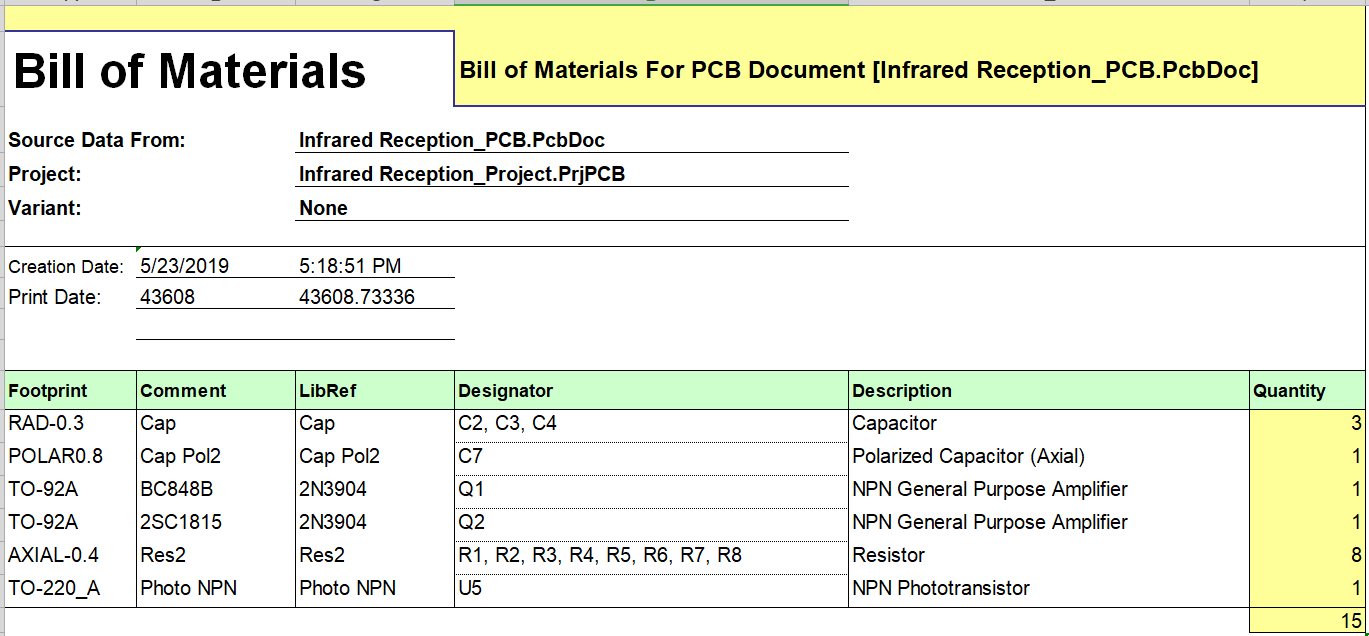
\includegraphics[width=1\textwidth]{7-2.png}
    \caption{红外接收PCB板元器件列表}
    \label{fig:xfig1}
 \end{figure}

 \subsection{管脚数量}
 \begin{figure}[H]
    \centering%
    \subcaptionbox{红外发射PCB板管脚数量\label{fig:subfig1}}[3cm] %标题的长度,超过则会换行,如下一个小图。
      {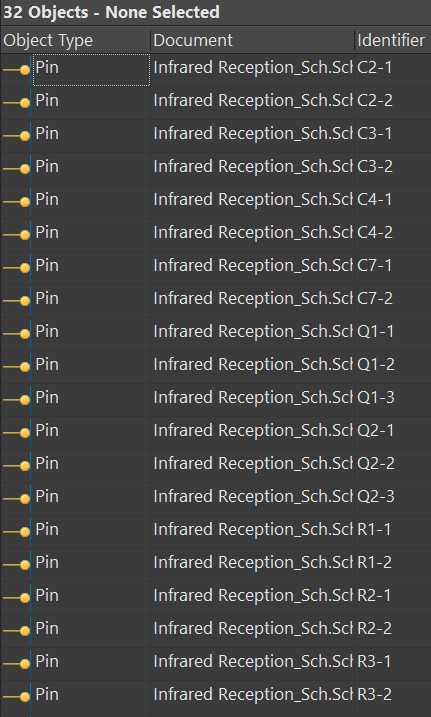
\includegraphics[width=0.3\textwidth]{8-1.png}}%
    \hspace{4em}%
    \subcaptionbox{红外接收PCB板管脚数量\label{fig:subfig2}}
        {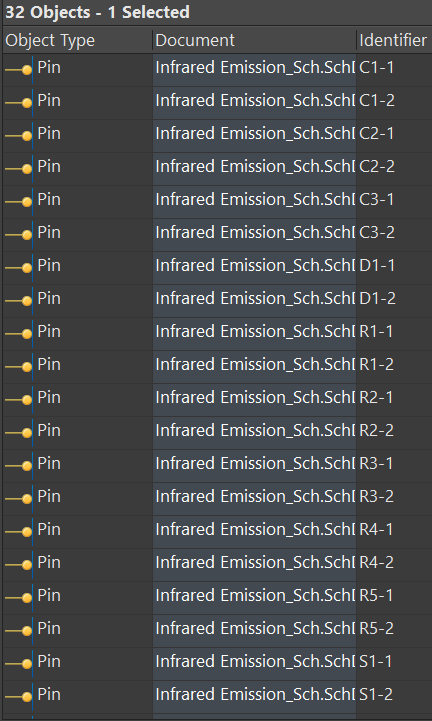
\includegraphics[width=0.3\textwidth]{8-2.png}}
    \caption{管脚数量}
    \label{fig:big1-subcaptionbox}
  \end{figure}
统计得到管脚数量为64根。

\subsection{进一步查看}

欢迎老师进行进一步的查看,附录中有\\

0. 论文写作的所有文件。以证明文章的原创性,需要使用Latex打开。
1. 原始版本的计划书\\
2. AD原理图以及PCB。里面有两个文件,分别时发射和接收,内有PCB和原理图源文件。\\
3. Multisim仿真及结果。里面有大量图片,均是仿真后的原图,文件需要使用Multisim14打开\\
4. 关键元器件手册。含有三个关键器件的芯片手册\\
非常希望老师能给出宝贵意见。随时可以联系我:812079716@qq.com。非常感谢老师!
